\documentclass[17pt,margin=1in,innermargin=-4.5in,blockverticalspace=-0.25in]{tikzposter}
\usepackage[rm]{roboto}
\usepackage[T1]{fontenc}
\geometry{paperwidth=42in,paperheight=30in}
\usepackage[utf8]{inputenc}
\usepackage{amsmath}
\usepackage{isu-theme}
\usepackage{amsfonts}
\usepackage{amssymb}
\usepackage{graphicx}
\usepackage{enumitem}
\usepackage{svg}
\usepackage[style=ieee,url=false,doi=false,isbn=false]{biblatex}

\addbibresource{./isu-ese.bib}


% set theme parameters
\tikzposterlatexaffectionproofoff
\usetheme{ISUTheme}
\usecolorstyle{ISUStyle}

\title{SIGMA: Systematic Island Grammar forMation Approach\\
Merging Grammars}
\author{Isaac Griffith and Rosetta Roberts}
\institute{Empirical Software Engineering Laboratory\\
College of Science and Technology, Idaho State University}

% begin document
\begin{document}
\maketitle
\centering
\begin{columns}
    \column{0.32}
    \block{Introduction}{
        Motivation---Many modern systems are written in multiple programming languages which are difficult to analyze.
        One approach to ease this process is to use multilingual island grammar parsers. In order to automate the
        process of creating multilingual island grammar parsers, one needs to automate merging grammars in a way
        that decreases their complexity and maintenance effort.

        Research Goal---We used the Goal-Question-Metric (GQM) paradigm \cite{caldieraGoalQuestionMetric1994} to form the 
        following research goal: Develop an automated approach for merging components of a grammar to facilitate
         the construction of both the island and water components in an island grammar in order to reduce both
          the overall initial effort required in creating such grammars and the effort required to 
          maintain such grammars.

        Research Question---To evaluate our automated approach, we formed two research questions.
        \begin{itemize}
            \item What is the effect that this process has on the effort of the merged grammars? -
            \textit{It is expected that this process decreases the maintenance effort.}
            \item What is the effect that this process has on the complexity of the merged grammars? - 
            \textit{It is expected that this process decreases the complexity.}
        \end{itemize}
    }
    \block{Approach}{
        \begin{minipage}[c]{.45\linewidth}
            \begin{center}
                Steps
            \end{center}
            \begin{enumerate}
                \item Parse Grammars
                \item Trivally Merge Grammars
                \item Normalize Grammar \label{normalize_step}
                \item Measure Production Similarities
                \item Merge Most Similar Productions \label{merge_similar_step}
                \item Repeat Steps \ref{normalize_step}--\ref{merge_similar_step} Until Max Similarity is Below a Threshold \label{threshold_step}
                \item Output Grammars
            \end{enumerate}
        \end{minipage}\hfill\begin{minipage}[c]{.5\linewidth}
            \begin{tikzfigure}[Merge Process]
                \label{fig:merge_process}
                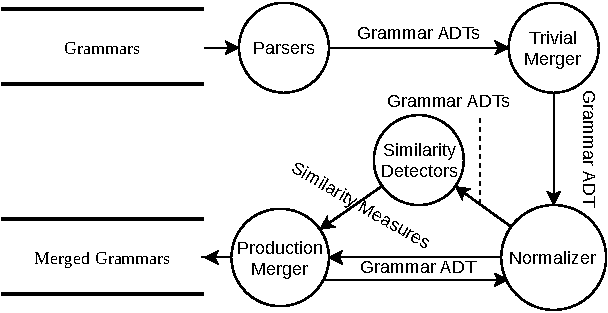
\includegraphics[width=\linewidth]{../../papers/merge/images/paper/SIGMA-DFD.pdf}
            \end{tikzfigure}
        \end{minipage}

        \begin{minipage}[c]{.55\linewidth}
            \begin{center}
                Data Model
            \end{center}
            SIGMA parses input grammars into the object oriented data model shown in figure \ref{fig:data_model}.
            The model is created by visiting each node of the grammar's abstract syntax tree. The grammar is
            recreated by visiting each object of the model.
        \end{minipage}\hfill\begin{minipage}[c]{.4\linewidth}
            \begin{tikzfigure}[Data Model]
                \label{fig:data_model}
                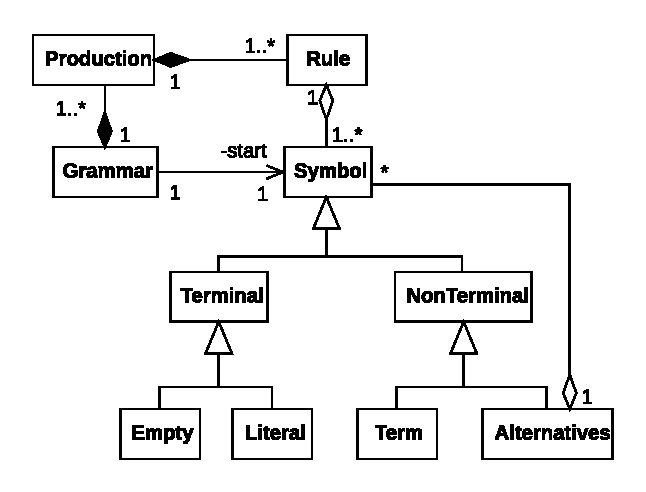
\includegraphics[width=\linewidth]{../../papers/merge/images/paper/diagram.eps}
            \end{tikzfigure}
        \end{minipage}%


        \innerblock{Measuring Production Similarity}{
            \begin{minipage}[t]{.49\linewidth}
                The similarity of productions $P_a,P_b$ that both expand to a sequence of 
                symbols $p_1p_2...$ is calculated by finding the Longest Common
                Subsequence (LCS) between the productions and then using the following formula.
                $$\frac{2|LCS(P_a, P_b)|}{|P_a|+|P_b|}$$
                
            \end{minipage}\hfill\begin{minipage}[t]{.49\linewidth}
                The similarity of productions $P_a,P_b$ that both expand to one of several
                symbols $p_1|p_2|...$ is calculated by finding the number of shared symbols
                and then using the following formula.
                $$\frac{2|P_a \cup P_b|}{|P_a|+|P_b|}$$
            \end{minipage}
        }
        
        \innerblock{Normalization}{
            SIGMA normalizes grammars so that all rules match one of two forms:

            \begin{center}
                \texttt{$\texttt{P}_1\rightarrow$ A`a'B}\\
                \texttt{$\texttt{P}_2\rightarrow$ A|`a'|B}
            \end{center}
        }
    }

    \column{0.36}
    \block{Experimental Design}{
        \begin{minipage}[t]{.33\linewidth}
            \begin{tikzfigure}[Data Collection Process]
                \label{fig:data-collect}
                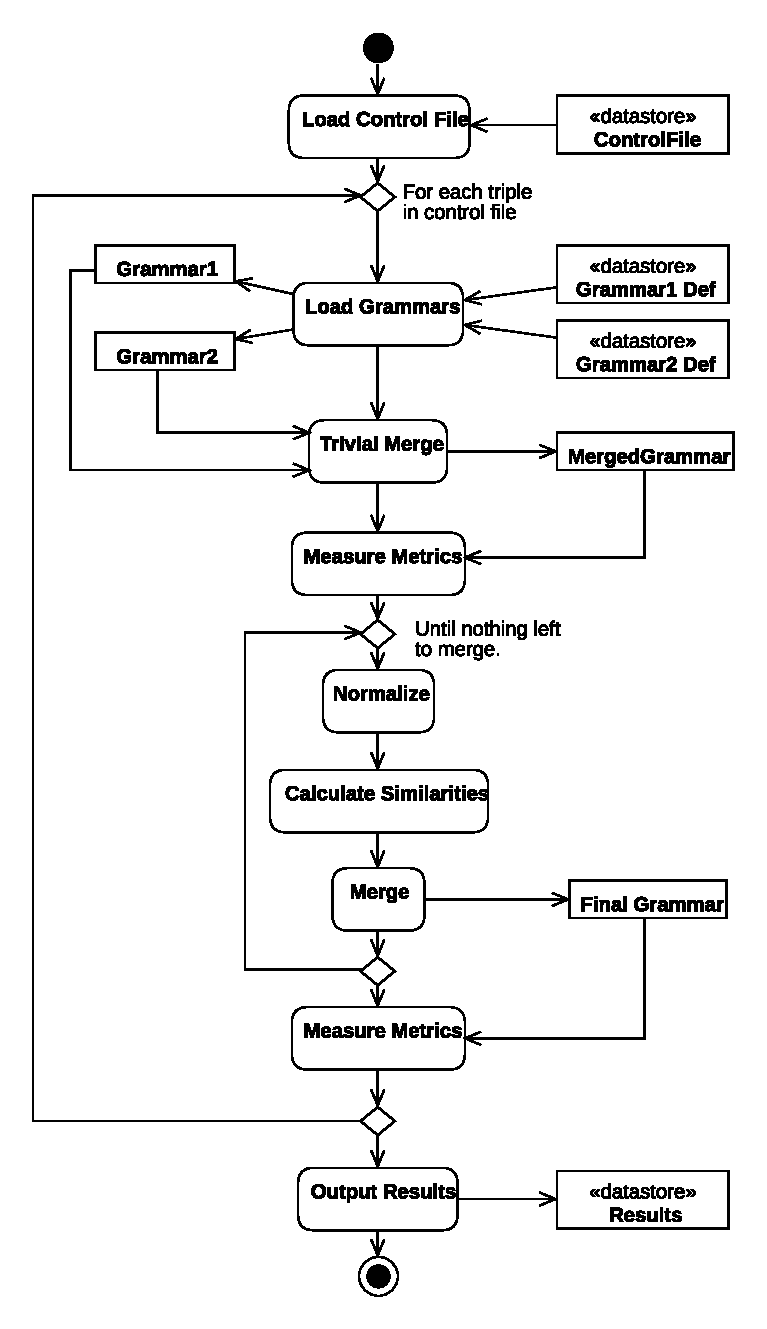
\includegraphics[width=\linewidth]{../../papers/merge/images/paper/data_collect.eps}
            \end{tikzfigure}
        \end{minipage}\hfill\begin{minipage}[t]{.67\linewidth}
            \begin{itemize}
                \item One Experiment for Each of $\Delta$HAL and $\Delta$MCC.
                \item 3*5 Factorial Design With 5 Repetitions
                \item Experimental Units --- To select our experimental units, we split
                grammars from the ANTLR4\footnote{\url{https://github.com/antlr/grammars-v4}} repository into 3 sizes, selected 12 grammars
                from each size category, and selected 50 unordered pairs of grammars from each
                size category.
                \item Threshold From Step \ref{threshold_step} of Approach. We used 5 different levels
                of our threshold: .01, .25, .5, .75, 1.0. A threshold of 1.0 was our control.
                \item Experimental Measures. From \cite{powerMetricsSuiteGrammarbased2004}.
                    \begin{itemize}
                        \item[PROD] Number of Productions. Measure of Size of Grammars.
                        \item[$\Delta$HAL] Amount Halstead Effort Decreased. Measure of the Maintainability of Grammars.
                        \item[$\Delta$MCC] Amount Cylomatic Complexity Decreased. Measure of Grammar Complexity.
                    \end{itemize}
                \item Analysis
                    \begin{itemize}
                        \item Permutation F-Test
                        \item Jonchheere-Terpstra Test
                        \item Steel Test
                    \end{itemize}
            \end{itemize}
        \end{minipage}
    }
    \block{Results}{
        \begin{minipage}[t]{.5\linewidth}
            \innerblock{$\Delta$HAL}{
                \begin{tikzfigure}[$\Delta$HAL Box Plot]
                    \centering
                    \label{fig:hal-box}
                    \includesvg[width=.66\textwidth]{../../data/merge/hal_box.svg}
                \end{tikzfigure}

                \begin{minipage}[c]{.5\linewidth}
                    \begin{center}
                        Interaction
                    \end{center}
                    \begin{itemize}
                        \item F --- 5.098
                        \item p --- 7.31e-05
                        \item Influential primarily at control
                    \end{itemize}
                \end{minipage}\hfill\begin{minipage}[c]{.5\linewidth}
                    \begin{tikzfigure}[$\Delta$HAL Interaction Plot]
                        \centering
                        \includesvg[width=\textwidth]{../../data/merge/ex1_interaction.svg}
                    \end{tikzfigure}
                \end{minipage}
                \begin{enumerate}
                    \item Perm. F-Test --- F: 9.569, p: 4.73e-06
                    \item JT Test --- Statistic: 767, p: 6e-4
                    \item Steel Test --- p:
                \end{enumerate}
            }
        \end{minipage}\hfill\begin{minipage}[t]{.5\linewidth}
            \innerblock{$\Delta$MCC}{
                \begin{tikzfigure}[$\Delta$MCC Box Plot]
                    \centering
                    \label{fig:hal-box}
                    \includesvg[width=.66\textwidth]{../../data/merge/mcc_box.svg}
                \end{tikzfigure}

                \begin{minipage}[c]{.5\linewidth}
                    \begin{tikzfigure}[$\Delta$MCC Interaction Plot]
                        \centering
                        \includesvg[width=\textwidth]{../../data/merge/ex2_interaction.svg}
                    \end{tikzfigure}
                \end{minipage}\hfill\begin{minipage}[c]{.5\linewidth}
                    \begin{itemize}
                        \item F --- 
                        \item p --- 
                        \item Influential primarily at control
                    \end{itemize}
                \end{minipage}
                \begin{enumerate}
                    \item Perm F-Test --- F: , p:
                    \item JT Test --- Statistic: , p:
                    \item Steel Test --- p:
                \end{enumerate}
            }

        \end{minipage}
    }
    
    \column{0.32}
    \block{Discussion}{
        \begin{itemize}
            \item Our experiment found that SIGMA's merging process reduced the complexity and the maintainability
            effort of grammars regardless of their size and the threshold used. This is confirmed by the Steel Test.
            \item As the threshold decreases, complexity and maintainability effort decreased as confirmed by
            the JT Test.
            \item There were significant interactions between the threshold and size. However, these were only
            present at our control.
        \end{itemize}
    }
    \block{Threats to Validity}{
        \begin{itemize}
            \item Internal --- We selected grammars from only the ANTLR4 grammar respository. Therefore our
            conclusions cannot necessarily be generalized past grammars in this repository. 
            \item External --- Our experimental units lacked grammars in formats commonly used in industry such
            as TXL, SDF, etc.
            \item Conclusion/Construct --- None
        \end{itemize}
    }
    \block{Conclusions}{
        We sucessfully created a tool that merges programming language grammars. This tool was demonstrated to 
        decrease the maintainability effort and complexity of grammars. Because this merging process has the qualities
        that we desire, it can be used as part of a larger process for automatically creating island grammars for
        multilingual parsing.
    }
    \block{Future Work}{
        Possible directions for future work include the following. We intend to investigate the normalization process
        to ensure each step is necessary. We plan to evaluate this method on the larger collection of grammars 
        GrammarZoo\cite{zaytsevGrammarZooCorpus2015}.  We also intend to integrate our
        approach with current approaches of creating tolerant grammars\cite{klusenerDerivingTolerantGrammars2003}.
        Finally we intend to augment our process with additional algorithms to allow it to automatically construct island grammars
        for multilingual parsing.
    }
    
    
    \block{References}{
        \begin{footnotesize}
        \printbibliography[heading=none]
        \end{footnotesize}
    }
    
    \block{Acknowledgements}{
        \begin{footnotesize}
            This research is supported by funding from the Ronald E. McNair Post Baccalaureate Achievement Program at Idaho State University, which is sponsored by the Department of Education (P217A170169).
        \end{footnotesize}
    }
\end{columns}
\end{document}